\documentclass[border=1cm]{standalone}
\usepackage{tikz}
\usetikzlibrary{positioning, shapes, calc}

\begin{document}
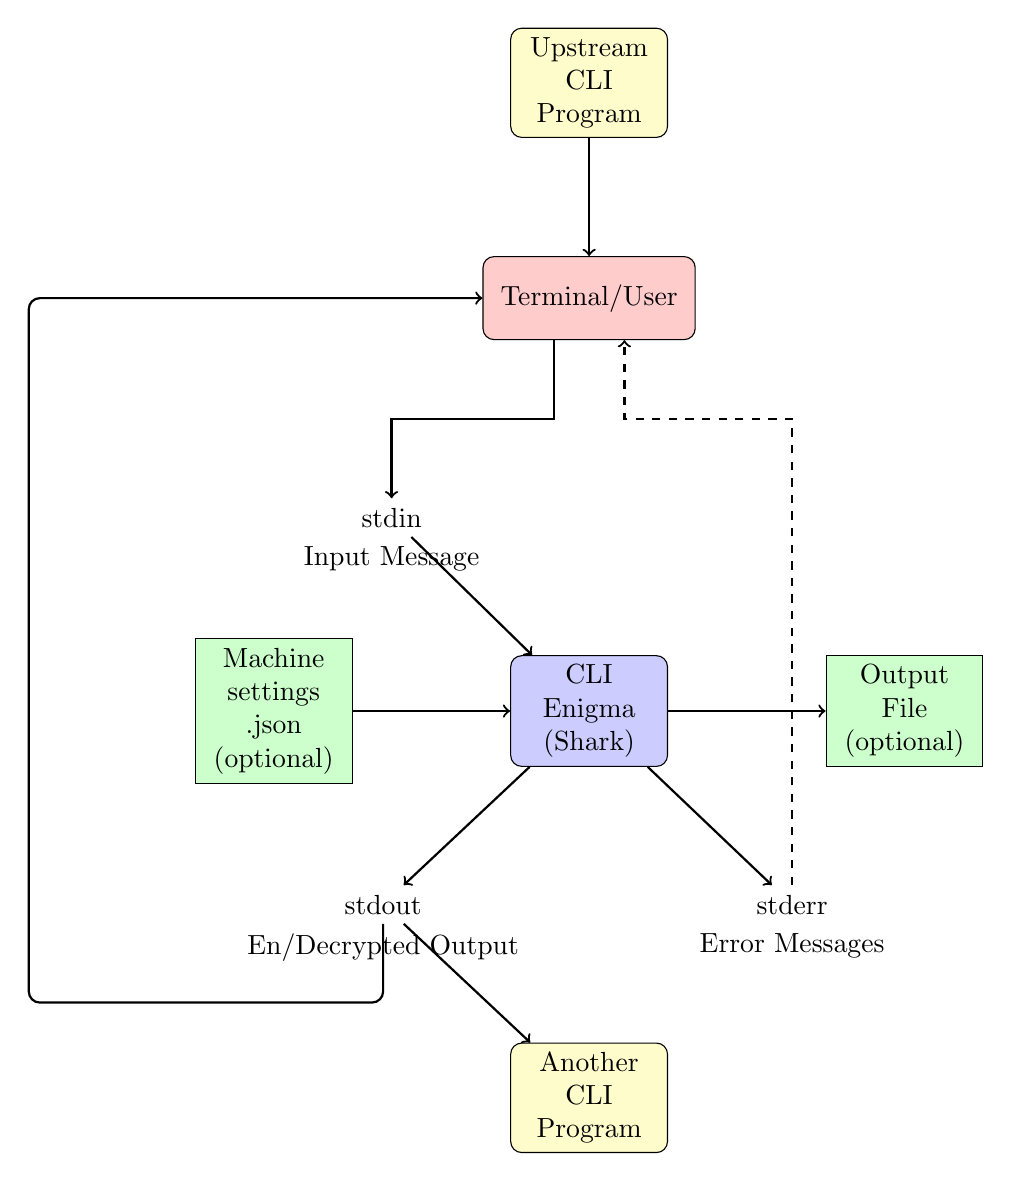
\begin{tikzpicture}[node distance=2cm,
                    block/.style={rectangle, draw, fill=blue!20, rounded corners, text width=5em, text centered, minimum height=2.5em},
                    file/.style={rectangle, draw, fill=green!20, text width=5em, text centered, minimum height=2.5em},
                    terminal/.style={draw, fill=red!20, shape=rectangle, text width=7em, text centered, rounded corners, minimum height=3em}]

    % Nodes
    \node[block] (cli) {CLI Enigma \\ (Shark)};

    \node[above left=1.5cm and 1cm of cli, label=below:Input Message] (stdin) {stdin};
    \node[left=of cli, file] (inputfile) {Machine settings .json \\ (optional)};
    \node[below left=1.5cm and 1cm of cli, label=below:En/Decrypted Output] (stdout) {stdout};
    \node[below right=1.5cm and 1cm of cli, label=below:Error Messages] (stderr) {stderr};
    \node[right=of cli, file] (outputfile) {Output File \\ (optional)};

    \node[above=4cm of cli, terminal] (terminal) {Terminal/User};
    \node[above=1.5cm of terminal, block, fill=yellow!20] (upstreamcli) {Upstream CLI Program};

    \node[below=3.5cm of cli, block, fill=yellow!20] (anotherprog) {Another CLI Program};

    % Paths
    \draw[->, thick] (stdin) -- (cli);
    \draw[->, thick] (inputfile) -- (cli);
    \draw[->, thick] (cli) -- (stdout);
    \draw[->, thick] (cli) -- (stderr);
    \draw[->, thick] (cli) -- (outputfile);
    \draw[->, thick] (terminal.230) -- ($(terminal.230)+(0,-1cm)$) -| (stdin);
    \draw[->, thick, dashed] (stderr) |- ($(terminal.310)+(0,-1cm)$) -- (terminal.310);
    \draw[->, thick] (stdout) -- (anotherprog);
    \draw[->, thick, rounded corners] (stdout.south) |- ++(-4.5cm,-1cm) |- (terminal.west);
    \draw[->, thick] (upstreamcli) -- (terminal);

\end{tikzpicture}
\end{document}